\chapter{Transient Noise Detection}\label{ch:TransientNoiseDetection}

\ifpdf
    \graphicspath{{Chapter5_TransNoiseDet/Chapter5Figs/PNG/}{Chapter5_TransNoiseDet/Chapter5Figs/PDF/}{Chapter5_TransNoiseDet/Chapter5Figs/}{Chapter5_TransNoiseDet/Chapter5Figs/NoiseBurstModel/}}
\else
    \graphicspath{{Chapter5_TransNoiseDet/Chapter5Figs/EPS/}{Chapter5_TransNoiseDet/Chapter5Figs/}}
\fi

The rapid increase in availability of high speed internet connections has made personal computers a popular basis for teleconferencing applications. While embedded microphones, loudspeakers and webcams in laptop computers have made setting up conference calls very easy, it has also brought with it some specific noise difficulties such as feedback, fan noise and button clicking noise. The latter has been a particularly persistent problem and is generally due to the mechanical impulses caused by keystrokes. Particularly on laptop computers this can be a significant nuisance due to the mechanical connection between microphone, within in the laptop case, and the keyboard, and the distinct tactile interface points throughout the key travel. The noise pulses produced can vary greatly with factors such as keystroke speed and length, microphone placement and response, laptop frame or base, keyboard or trackpad type and even surface on which the computer is placed.

The focus of our noise reduction efforts will purely be on the perspective of the receiving end since this is the only noise accessible to us through signal processing, but also since the acoustical feedback from keyboards is often an important cue for the typer, whereas to the receiver it will uncorrelated with any actions.

As noted in the literature review, chapter~\ref{sec:LitRev_Detection}, a range of approaches has been taken to detect impulsive noise in speech and audio. In general the approaches taken can be divided into two categories. The ones that focus on corruptions caused by mechanical defects in the medium or errors in the communication channel and \todo{finish}

\section{A look at the data}
Figure~\ref{fig:TypingSPLKeyboards} shows a plot of the A-weighted sound pressure level (SPL) of 4 different keyboard impulses aligned\cite{Hauswirth2013}. This data was recorded with an artificial binaural head measurement system in an anechoic environment and as such only serves to outline audible real world acoustic scenario of keystroke impulses. The data clearly shows some key features of keyboard noise.
\begin{enumerate}
\item The length of keyboard strokes can be upwards of 350 ms.
\item In all tested cases the impulses consist of at least 2 clearly defined pulses.
\item The majority of the energy lies in the initial pulse.
\end{enumerate}

The number 2 pulse seen for every device in Figure~\ref{fig:TypingSPLKeyboards} shows what will be referred to as the \emph{lift} pulse from this point onwards. This pulse is related to the physical key or switch returning to its original unpressed position. The relationship between the two pulses are not consistent across different devices and Laptop 1 specifically was said to have a ``hard return stop'' while Laptop 3 has a ``soft return stop'' with a SPL level difference of almost nothing and 18 dB(A) SPL respectively.

\begin{figure}[!] %TypingSPLKeyboards
\centering
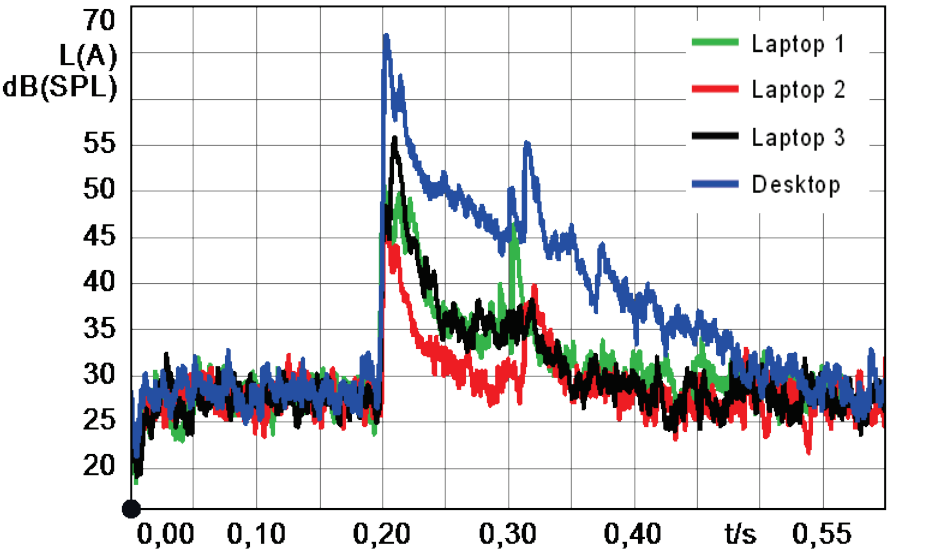
\includegraphics[width=100mm]{TypingSPLKeyboards.png}
\caption{SPL analysis of keyboard noise (time weighting: 2ms). Plot reproduced from \cite{Hauswirth2013}.}\label{fig:TypingSPLKeyboards}
\end{figure}

Figure~\ref{fig:TypingLoudnessKeyboards} shows the loudness of keyboard impulses versus time. Loudness is a representation of a human's perception of sound volume and is represented on a linear scale so that twice the loudness represents a listener perceiving the sound twice as loud. The figure shows that the desktop keyboard is perceived as being over twice as loud as a laptop keyboard. Desktop keyboards are traditionally optimised for typing comfort and tactile feedback while not having to consider the spacial constraints of laptop computers. In addition some keyboards are specifically designed to give the user audible feedback\cite{Hauswirth2013}.

\begin{figure}[!] %TypingLoudnessKeyboards
\centering
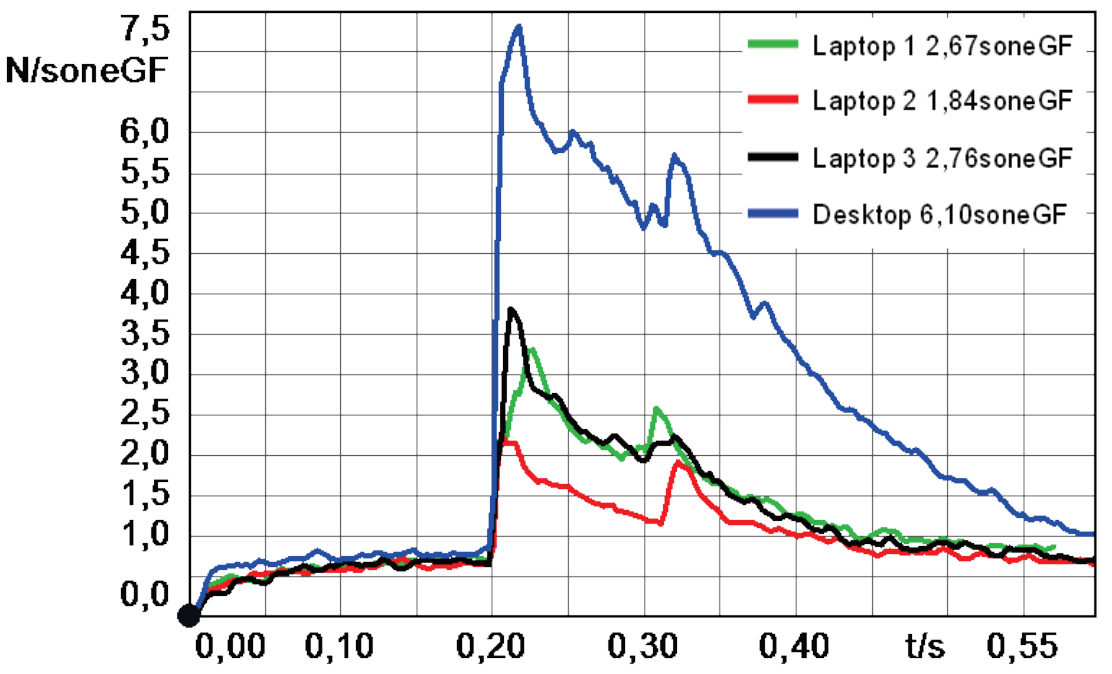
\includegraphics[width=100mm]{TypingLoudnessKeyboards.png}
\caption{Loudness analysis of keyboard noise. Plot reproduced from \cite{Hauswirth2013}.}\label{fig:TypingLoudnessKeyboards}
\end{figure}

In addition to the loudness, Figure~\ref{fig:TypingLoudnessKeyboards} also shows the 5\% percentile value as a single number in the diagram legend. This value indicated the value which the signal exceeds during 5\% of the examined time interval\cite{Hauswirth2013}. This number also reflects the fact that the desktop keyboards in general are perceived much more loudly than laptop keyboards so while laptop keyboards are of interest due to their mechanical connection and physical proximity to the microphone, desktop keyboards is clearly also a potential source of nuisance in telecommunication applications.

\subsection{Spectral investigation of audio signals}
Figure~\ref{fig:spectrogramMarkedTapsBrownFox} shows a spectrogram of a short sequence of speech with typing strokes embedded in it. The figure overlays show the approximate positions of the strokes in the spectrogram. It can be observed that the typing strokes have a fairly flat frequency response compered to the the voiced parts of the audio sequence.

\begin{figure}[!] %spectrogramMarkedTapsBrownFox
\centering
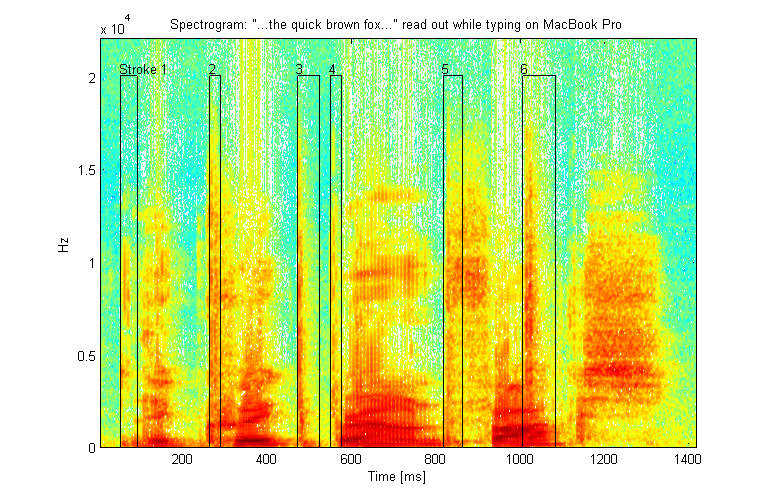
\includegraphics[width=150mm]{spectrogramMarkedTapsBrownFox.png}
\caption{Spectrogram analysis of mixed typing strokes and speech. Overlay shows positions of typing strokes.}\label{fig:spectrogramMarkedTapsBrownFox}
\end{figure}

Figure~\ref{fig:waveletspectrumAno} shows the wavelet spectrum of a sequence of keystrokes with speech interference. The figure overlays show the approximate positions of the strokes in the wavelet spectrum.
\begin{figure}[!] %waveletspectrumAno
\centering
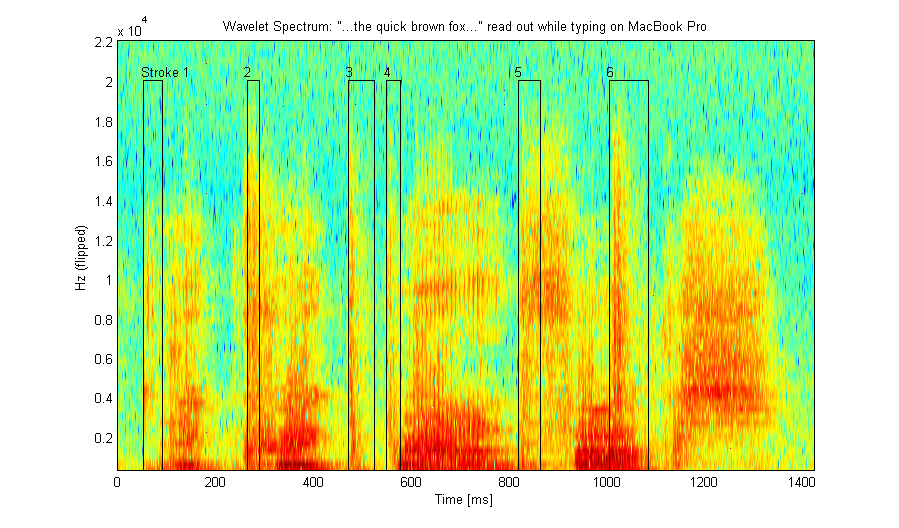
\includegraphics[width=150mm]{waveletspectrumAno.png}
\caption{Top: Waveform of typing sequence. Bottom: Wavelet spectrum of same typing sequence.}\label{fig:waveletspectrumAno}
\end{figure}

\subsection{Keystroke sequence investigation}
A single keystroke, during rapid typing and not at the end of a typing sequence, is generally made up of 3 primary sections.
\begin{enumerate}
  \item A primary \textbf{Stroke} keystroke (15 - 40 ms),
  \item a \textbf{Break} while key is depressed (50 - 500 ms) and
  \item a \textbf{Lift} impulse (15 - 40 ms).
\end{enumerate}
The duration of the break region will typically be determined by the typing speed of the user while the Stroke and the Lift region are primarily constant and will vary more with factors such as stroking force and the vibrational characteristics of the keyboard and the laptop casing.

Figure~\ref{fig:KeyboardStrokeSlow} shows a waveform of a single typing stroke. The waveform clearly shows the two distinct impulses of sudden erratic excitation followed by a slowly decaying low frequency sinusoid.

\begin{figure}[!] %KeyboardStrokeSlow
\centering
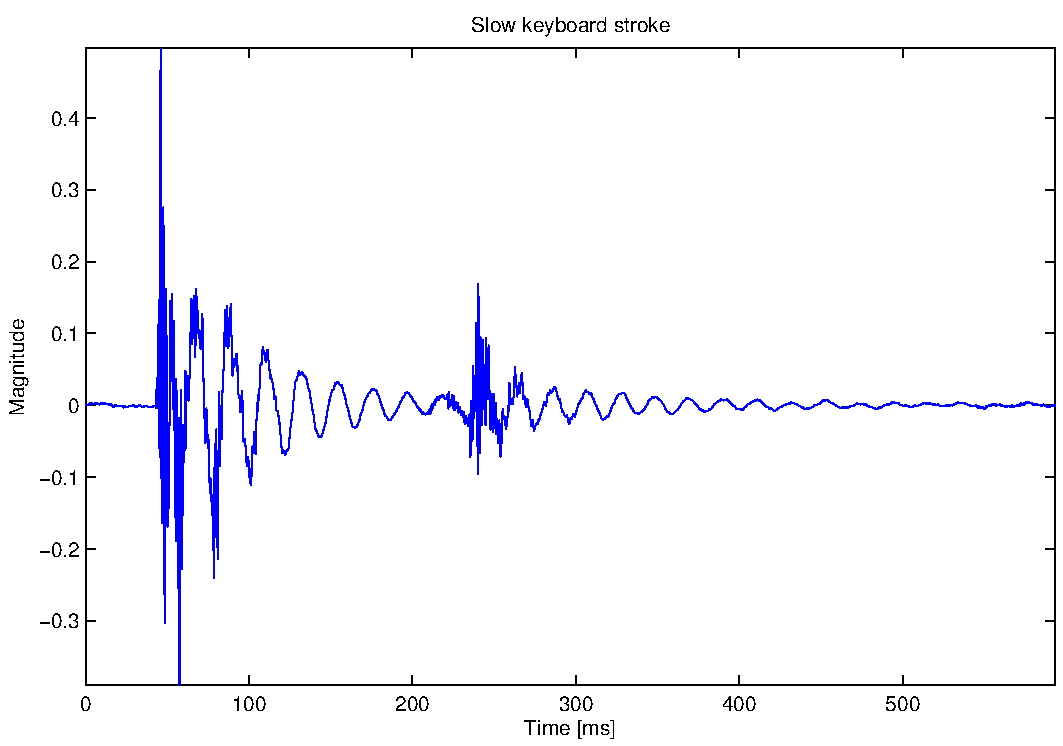
\includegraphics[width=120mm]{KeyboardStrokeSlow.pdf}
\caption{Single slow keyboard stroke.}\label{fig:KeyboardStrokeSlow}
\end{figure}

Figure~\ref{fig:Keyboard2StrokesFast} shows a sequence of two keystrokes in rapid succession. The keystroke regions mentioned above are clearly annotated with their temporal extent also noted.

\begin{figure}[!] %Keyboard2StrokesFast
\centering
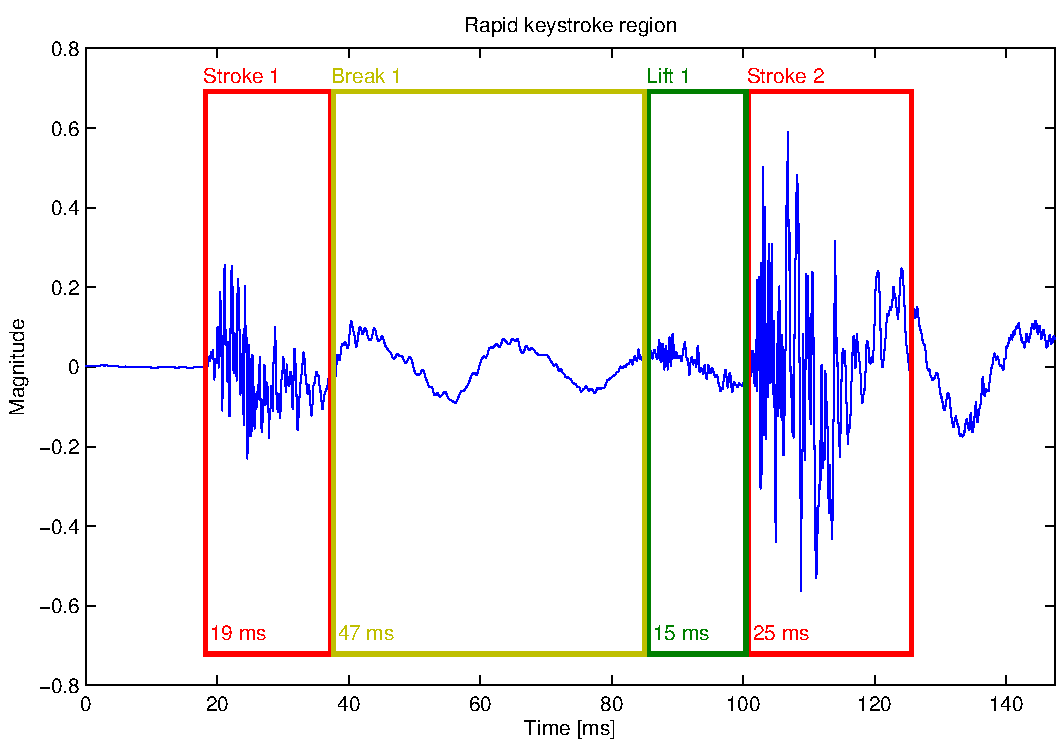
\includegraphics[width=120mm]{Keyboard2StrokesFast.pdf}
\caption{Two annotated keyboard strokes in rapid succession.}\label{fig:Keyboard2StrokesFast}
\end{figure}

Figure~\ref{fig:Keyboard4StrokesFast} shows an example of a short rapid 4 keystroke sequence.

\begin{figure}[!] %Keyboard4StrokesFast
\centering
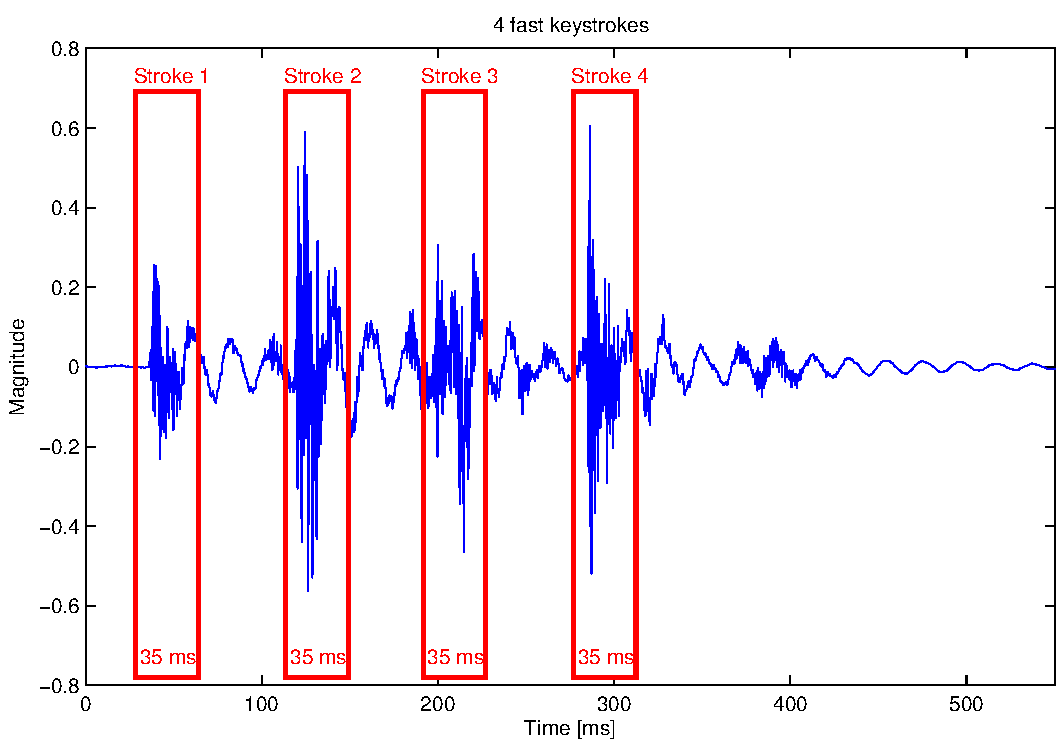
\includegraphics[width=120mm]{Keyboard4StrokesFast.pdf}
\caption{Four annotated keyboard strokes in rapid succession.}\label{fig:Keyboard4StrokesFast}
\end{figure}

\section{Detection algorithms}\label{sec:WPdetection}

The basic detection algorithm is comprised of two stages. First a separation stage aims to separate the transient noise pulses by separating out tonal atoms assumed to be speech components and secondly a detection stage which attempts to detect transient noise events through the wavelet bases. For the detection stage 2 different approaches has been explored.

\subsection{Separation pre processing}
The incoming audio signal can be expressed as the linear combination of a voiced signal and a sparse signal containing the transient noise events:
\begin{equation}\label{eq:modelgeneral}
    x(n) = \sum_i c_i \Phi_i(n) + \sum_{j} w_{j}(n) \Psi_{j}(n),
\end{equation}
where $c_i$ are the coefficients for the voiced parts of the signal and $\Phi$ is the standard short-time Fourier basis. $w_{j}(n)$ are the coefficients of the residual where $j$ is an integer relating to some translation and dilation of some Wavelet basis function $\Psi$. Here we are utilising an overcomplete dictionary of atoms to represent the audio: a dictionary of `tonal' atoms and a dictionary of `transient' atoms that are aimed at capturing voiced speech and transient noise, respectively. Multiple dictionaries have been employed in Bayesian probabilistic methodologies for noise reduction purposes in \cite{Fevotte2006}\cite{Fevotte2008} (see also references therein for other approaches with multiple dictionaries). \todo{Maybe remove this: }We plan to report on such fully Bayesian approaches to our model above in future publications, but here we focus on development of a fast algorithm using the principles of the above model in order to first extract the tonal (voiced) components in order to process the noise components directly in wavelet domain. Other tonal dictionaries such as Gabor functions and other transient dictionaries such as standard discrete or continuous wavelet transforms can of course be substituted in our methods with minor modifications. Wavelets are found to be particularly suited to the types of noise transient we observe here, which are localised in time and can be of highly variable durations and frequency profile.

The coefficients $w_{j}(n)$ from equation (\ref{eq:modelgeneral}) can be interpreted as wavelet coefficients from a Wavelet Packet Decomposition (WPD) such that $j$ denotes the $j$th terminal node or scale, $j \in \{1, \ldots, J\}$ where $J = L^2$ for an level $L$ decomposition, and $n$ is the time index related to the coefficient set and so $w(n)$ will be used to denote a vector of all coefficients at a given time index $n$. For the case of a wavelet decomposition with decimation steps the time index from the terminal node coefficient sets and equation~\ref{eq:modelgeneral} will be related by a factor of $1/J$.




\subsubsection{Algorithm description}
The method for selecting the tonal components from the noisy signal is described in this section.

As described in the literature\todo{cite literature on speech modelling}, speech signals are typically slowly varying signals with energy concentrated around specific frequencies known as formant frequencies. These frequencies are related to the physiological shape of the human vocal tract and are typically manifested as spectral peaks\cite{Fant1970}. The algorithm attempts to detect these peaks and separate out this presumed vocal content. Figure~\ref{fig:Separation_Spectrum_Selection.pdf} shows an example of the algorithm running on block of speech data. A diagrammatic representation of the algorithm is shown in Figure~\ref{fig:SeparationDiagram.pdf} where ``iSTFT'' refers to the inverse Fourier transform on a windowed block of data.

\begin{figure} %Separation_Spectrum_Selection.pdf
\begin{minipage}[b]{1.0\linewidth}
  \centering
  \centerline{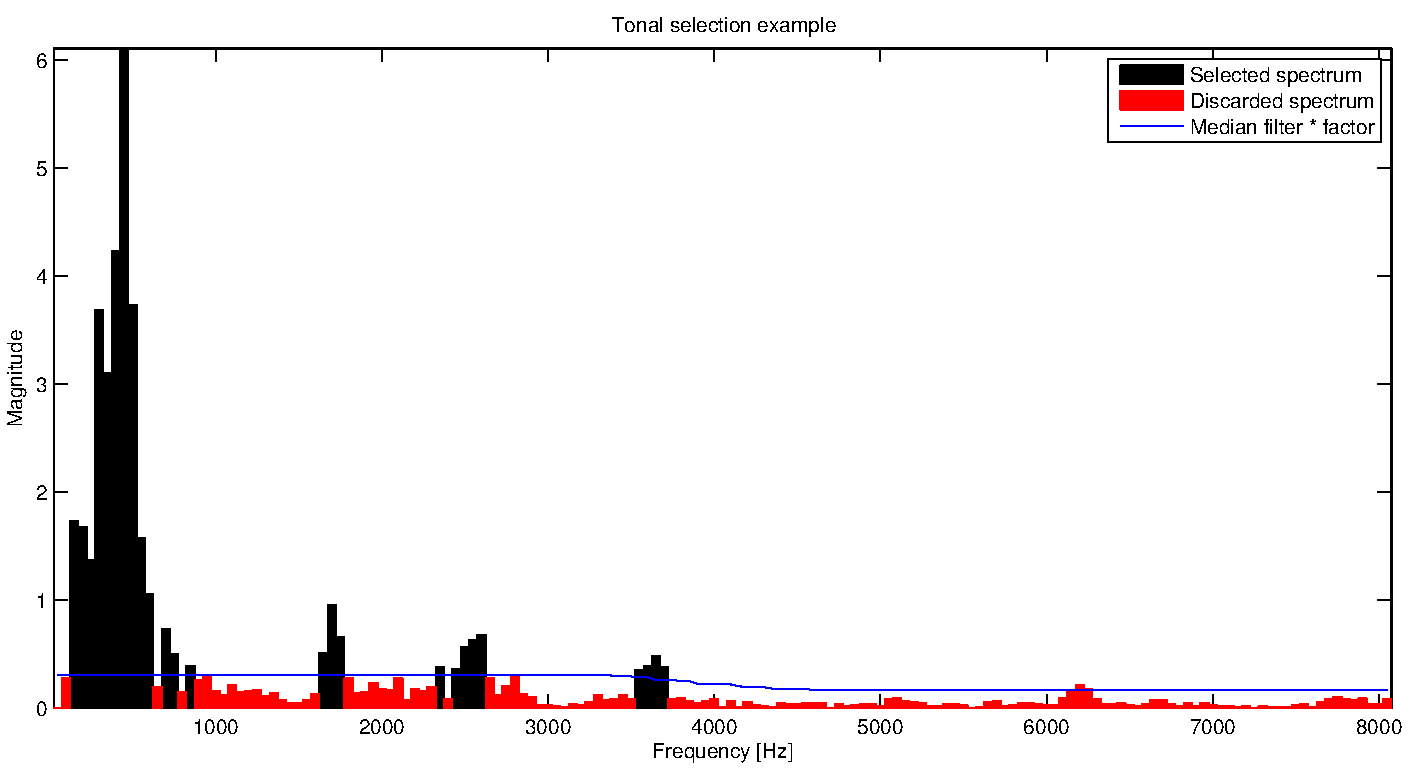
\includegraphics[width=14cm]{Separation_Spectrum_Selection.pdf}}
\end{minipage}
\caption{Example of the tonal selection algorithm. Block size of 320 samples. Audio sample rate of 16kHz.}
\label{fig:Separation_Spectrum_Selection.pdf}
\end{figure}

The algorithm proceeds by calculating a running median value of the STFT magnitude coefficients from a 320 sample long signal buffer. The media filter takes the running median value of 60 spectral samples and coefficients exceeding some factor $\nu$ of the median value (blue line in figure) are selected as tonal values (black bars). The red bars in Figure~\ref{fig:Separation_Spectrum_Selection.pdf} are assumed to be transient noise and their magnitude is set to zero. A suitable factor of the median value needs to be selected and for this application $\nu = 3.5$ was chosen. The detection of formant frequencies were additionally confined to be above 85 Hz and below 4000 Hz.

\begin{figure} %SeparationDiagram.pdf
\centering
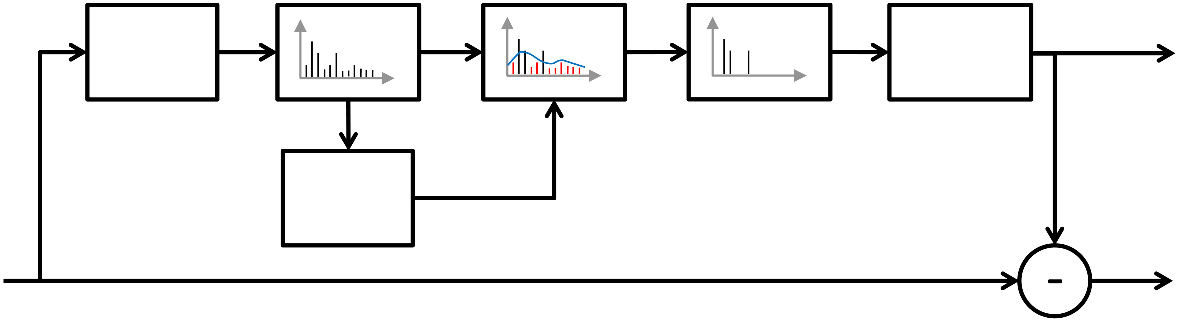
\includegraphics[width=140mm]{SeparationDiagram.pdf}
\begin{picture}(0,0)
\put(-420,20){Signal}
\put(-30,97){Tonal}
\put(-30,20){Residual}

\put(-302,45){Median}
\put(-302,30){filter}

\put(-362,88){STFT}
\put(-90,88){iSTFT}
\end{picture}
\caption{Diagram of separation algorithm.}
\label{fig:SeparationDiagram.pdf}
\end{figure}

\todo{This is a bit weak?}
A proposed addition to the algorithm described above and represented in Figure~\ref{fig:SeparationDiagram.pdf} includes a step to replace removed spectral information in frames suspected of being corrupted by key strokes to make the tonal component itself sound better. First of all a simple detection algorithm is employed to detect the spectral characteristics of an impulse. For the purpose of this implementation the detection criteria was a certain proportion of energy in a high frequency band in relation to a low frequency band, since energy in speech frames is largely located at the lower frequencies while impulses exhibit a wider frequency response. Figure~\ref{fig:SeparationDiagram2.pdf} shows a diagram of the revised algorithm. The removed spectral components in a corrupted frame is replaced by components from a historic buffer containing uncorrupted data.


\begin{figure} %SeparationDiagram2.pdf
\centering
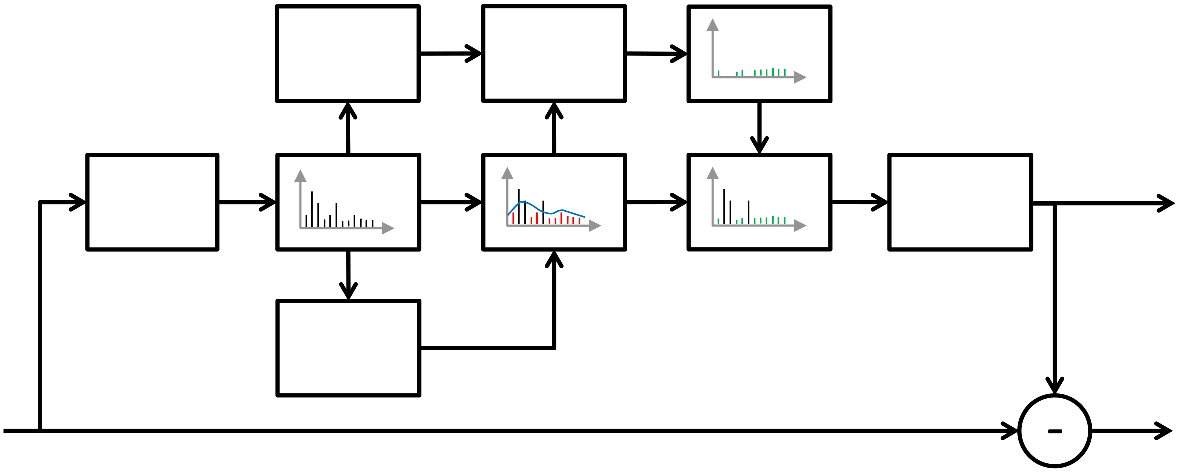
\includegraphics[width=140mm]{SeparationDiagram2.pdf}
\begin{picture}(0,0)
\put(-420,20){Signal}
\put(-30,97){Tonal}
\put(-30,20){Residual}

\put(-301,45){Median}
\put(-301,30){filter}

\put(-305,146){Simple}
\put(-305,131){Detector}

\put(-233,146){Vocal}
\put(-233,131){Memory}

\put(-362,88){STFT}
\put(-90,88){iSTFT}
\end{picture}
\caption{Diagram of separation algorithm.}
\label{fig:SeparationDiagram2.pdf}
\end{figure}

\subsubsection{Results}

Figure~\ref{fig:Separation_Residual_Example} shows an example of the residual obtained by simply subtracting outstanding peaks from the spectrum on frames of 20ms with 10ms overlap. The spectral peaks were identified using a threshold of a factor of three of the median filtered spectrum excluding frequencies below 85 Hz and above 10 kHz. The audio data presented in Figure~\ref{fig:Separation_Residual_Example} is a short sentence with two keystrokes embedded in it. The red plot overlay shows the residual where it is clear that the speech magnitude has been greatly reduced while the two clear keystrokes are largely left unchanged. \todo{Numerical justification for the effectiveness of the separation.}

\begin{figure}
\begin{minipage}[b]{1.0\linewidth}
  \centering
  \centerline{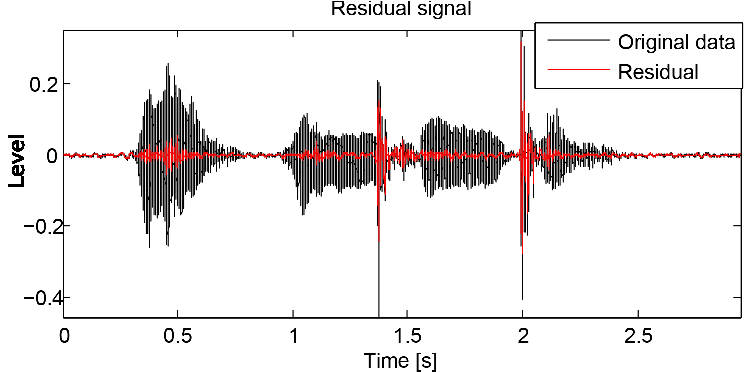
\includegraphics[width=10cm]{Separation_Residual_Example}}
\end{minipage}
\caption{Example of the separation step.}
\label{fig:Separation_Residual_Example}
\end{figure}

An example of the waveforms from the separation processing stage with both the tonal and the residual component zoomed in on a keyboard stroke plotted together, can be seen in Figure~\ref{fig:SeparationWaveformEx320.pdf}a and Figure~\ref{fig:SeparationWaveformEx320.pdf}b respectively. The data displayed in Figure~\ref{fig:SeparationWaveformEx320.pdf} is processed by applying the separation algorithm over blocks of 320 samples and sampled at 16kHz which is equivalent to blocks of 20ms, a common block size in communication systems\cite{Subramanya2007}. While the separation stage clearly removes the initial impulse, a strong tonal component of the keyboard typing pulse is retained and a lower frequency impulse, presumably related to the keyboard stroke, is also retained later in the example. 

\begin{figure} %SeparationWaveformEx320.pdf
\begin{minipage}[b]{1.0\linewidth}
  \centering
  \centerline{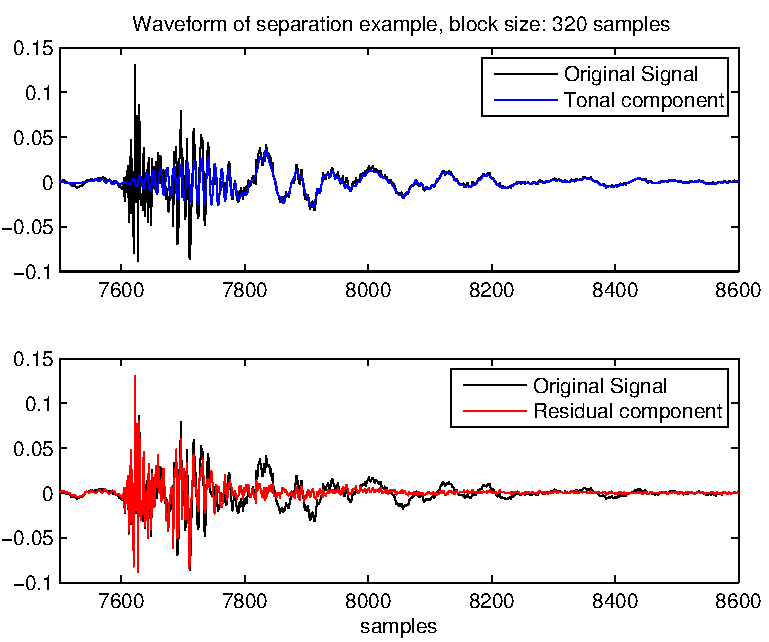
\includegraphics[width=12cm]{SeparationWaveformEx320.pdf}
  \begin{picture}(0,0)
\put(-310,270){a)}
\put(-310,130){b)}
\end{picture}}
\end{minipage}
\caption{Separation example of keyboard impulse, a) Tonal component, b) residual component. Sample rate: 16kHz. Block size: 320.}
\label{fig:SeparationWaveformEx320.pdf}
\end{figure}

Applying the algorithm to block sizes of 640 samples yields a better separation result as seen in Figure~\ref{fig:SeparationWaveformEx640.pdf}. Within blocks of 320 samples the tonal components of keyboard impulses may contain enough energy to make a significant impression on the spectrum to be detected as a tonal component but with a block size of 640 samples it is clear that less of the energy introduced by the keyboard stroke is retained.

\begin{figure} %SeparationWaveformEx640.pdf
\begin{minipage}[b]{1.0\linewidth}
  \centering
  \centerline{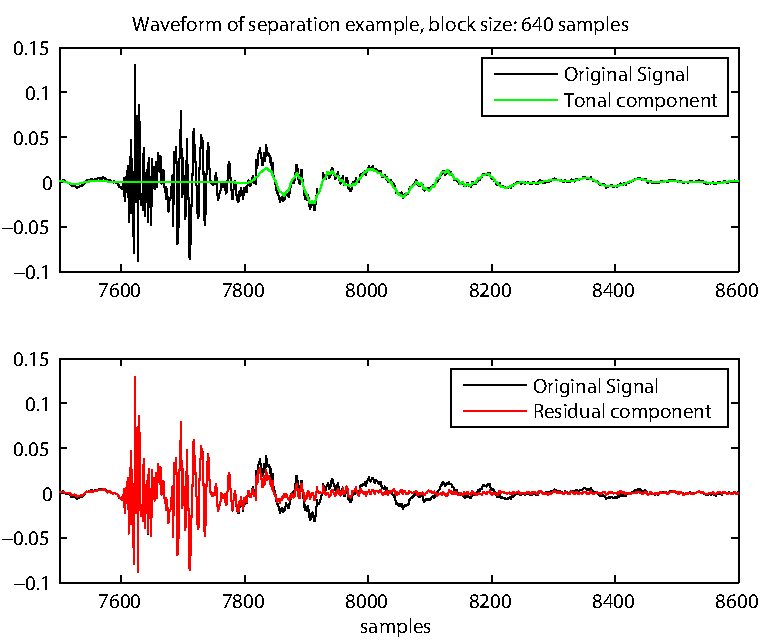
\includegraphics[width=12cm]{SeparationWaveformEx640.pdf}
  \begin{picture}(0,0)
\put(-310,270){a)}
\put(-310,130){b)}
\end{picture}}
\end{minipage}
\caption{Separation example of keyboard impulse, a) Tonal component, b) residual component. Sample rate: 16kHz. Block size: 640.}
\label{fig:SeparationWaveformEx640.pdf}
\end{figure}

In Figure~\ref{fig:SeparationWaveformExBig320.pdf} and \ref{fig:SeparationWaveformExBig640.pdf} a the keyboard strokes from Figure~\ref{fig:SeparationWaveformEx320.pdf} and \ref{fig:SeparationWaveformEx640.pdf} are seen with speech data. For both block sizes it is seen that the voiced parts of the signal are mainly represented in the tonal component while the keyboard stroke, around sample number 7600, is largely within the residual component. 

\begin{figure} %SeparationWaveformExBig320.pdf
\begin{minipage}[b]{1.0\linewidth}
  \centering
  \centerline{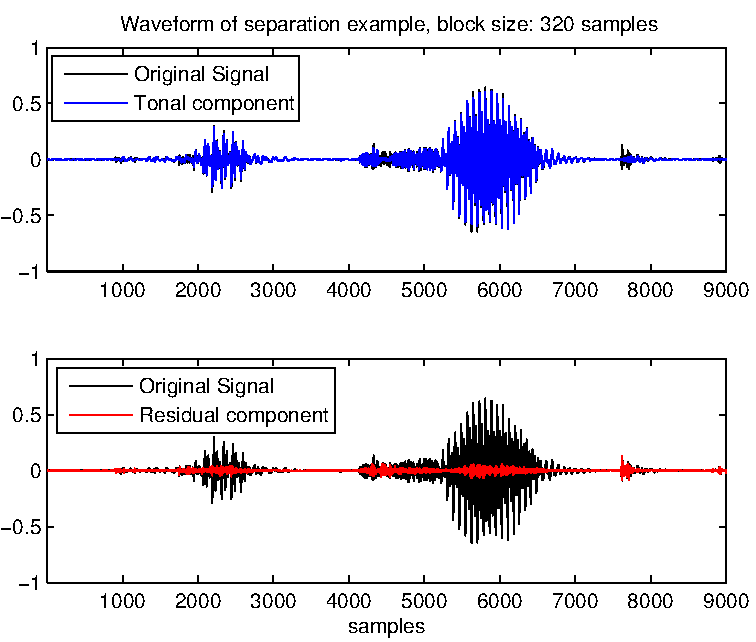
\includegraphics[width=12cm]{SeparationWaveformExBig320.pdf}
  \begin{picture}(0,0)
\put(-310,275){a)}
\put(-310,135){b)}
\end{picture}}
\end{minipage}
\caption{Separation example of speech and impulses, a) Tonal component, b) residual component. Sample rate: 16kHz. Block size: 320.}
\label{fig:SeparationWaveformExBig320.pdf}
\end{figure}

\begin{figure} %SeparationWaveformExBig640.pdf
\begin{minipage}[b]{1.0\linewidth}
  \centering
  \centerline{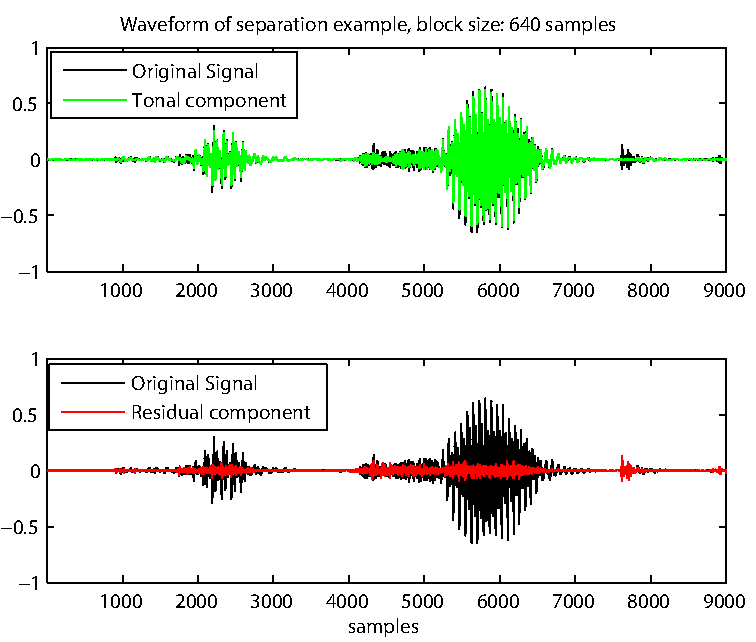
\includegraphics[width=12cm]{SeparationWaveformExBig640.pdf}
  \begin{picture}(0,0)
\put(-310,275){a)}
\put(-310,135){b)}
\end{picture}}
\end{minipage}
\caption{Separation example of speech and impulses, a) Tonal component, b) residual component. Sample rate: 16kHz. Block size: 640.}
\label{fig:SeparationWaveformExBig640.pdf}
\end{figure}

\subsection{Noise burst model}
We assume that the coefficients for each terminal node $j$ can be modeled as some switched additive noise process such that:

\begin{equation}\label{eq:model1}
    w_{j}(n) = i_{n} \theta_{n,j} + v_{n,j},
\end{equation}
where $i_{n}$ is the binary (1/0) switching variable denoting the presence of $\theta_{n,j}$ for $i_{n} = 1$ and otherwise $i_{n} = 0$. The transient signal $\theta_{n,j}$ is thus a switched noise burst corrupted by additive noise $v_{n,j}$.
Note that the grouping of the transient noise bursts will depend on the statistics of $i_{n}$ so that it is most likely that detections occur clusters. could be modeled as a Markov chain which will describe some degree of cohesion between frequency and time, i.e. the transient noise pulses will typically have a similar index of onset and will likely stay active for a length of time proportional with wavelet scale $j$.

We can now express our model in terms of the additive noise and a matrix of coefficients

\begin{equation}\label{eq:model2}
\boldsymbol{w} = \boldsymbol{\theta} + \boldsymbol{v},
\end{equation}

where $\boldsymbol{w} = [\boldsymbol{w}_1,\boldsymbol{w}_2,\ldots,\boldsymbol{w}_J]$ and where $\boldsymbol{w}_j = [w_{1,j}, w_{2,j}, \ldots, w_{N,j}]^T$ for the $j$th set of coefficients. $\boldsymbol{\theta}$ is the corresponding switched noise burst $J$ by $N$ matrix containing elements $i_{n}\theta_{n,j}$ and $\boldsymbol{v}$ is the random additive noise describing, for example, the effect of speech on the coefficients. For simplicity we consider $i_{n}$ to be constant across scales $j$ so the discrete vector $\boldsymbol{i} = [i_{1}, i_{2}, \ldots, i_{N}]$ can take any one of $2^{N}$ values. It is although possible to let $i$ vary with $j$ to express different detection characteristics at different scales. The detection task now becomes the estimation of the true state of $\boldsymbol{i}$ from the observed sequence $\boldsymbol{w}$.

Assuming that both the noise burst $\boldsymbol{\theta}$ and the background noise $\boldsymbol{v}$ can be modeled as zero mean Gaussian distributions, we have that:

\begin{equation}\label{eq:burst}
\boldsymbol{\theta}_n \sim \mathcal{N}_{\boldsymbol{\theta}_n}(0,\Lambda),
\end{equation}

where $\Lambda$ is a covariance matrix, here taken as diagonal with diagonal elements $\left[\lambda_{1}, \lambda_{2}, \ldots, \lambda_{J}\right]$, learned from training examples of keyboard clicks.

The background noise is also modelled as a zero-mean Gaussian process so that:

\begin{equation}\label{eq:noise}
\boldsymbol{v}_n \sim \mathcal{N}_{\boldsymbol{v}_n}(0,C_{\boldsymbol{v}}),
\end{equation}

where again $C_v$ is a diagonal covariance matrix with diagonal components \\*$[\sigma_{v,1}^2, \sigma_{v,2}^2, \ldots, \sigma_{v,J}^2]$.

%Bayes'
Treating the detection state $\boldsymbol{i}$ as a discrete random vector the probability of $\boldsymbol{i}$ conditional upon the observed (and corrupted) data $\boldsymbol{w}$ and other prior information available to us. This posterior probability $p(\boldsymbol{i}|\boldsymbol{w})$ can be expressed using Bayes' rule so that

\begin{equation}\label{eq:Bayes}
p(\boldsymbol{i}|\boldsymbol{w}) = \frac{p(\boldsymbol{w}|\boldsymbol{i})p(\boldsymbol{i})}{p(\boldsymbol{w})}
\end{equation}

where the likelihood $p(\boldsymbol{w}|\boldsymbol{i})$ will be a significant component of $p(\boldsymbol{i}|\boldsymbol{w})$.
$\boldsymbol{\theta}$ is our switched random noise process and its amplitude is defined by the noise burst amplitude p.d.f. $p_{\boldsymbol{\theta}}$ which is the joint distribution for the burst amplitudes where $i_{n} = 1$.

Since both functions $p_{\boldsymbol{v}}(\boldsymbol{v})$ and $p_{\boldsymbol{\theta}}(\boldsymbol{\theta})$ are zero-mean Gaussians, we can express each set of wavelet coefficients as $w_j(n)$ as:

\begin{equation}\label{eq:cases}
  w_j(n) \sim
  \begin{cases}
    \mathcal{N}(0,\sigma_{v,j}^2 + \lambda_j), & \quad i_n = 1\\
   \mathcal{N}(0,\sigma_{v,j}^2), & \quad i_n = 0,
  \end{cases}
\end{equation}

and the likelihood function $p(\boldsymbol{w}|\boldsymbol{i})$ becomes

\begin{equation}\label{eq:likelihood1}
p(\boldsymbol{w}|\boldsymbol{i}) = \prod^J \prod^N \mathcal{N}(0,\sigma_{v,j}^2 + i_n\lambda_j).
\end{equation}

The Maximum Likelihood (ML) estimate for $i_n$ can now trivially be calculated as
\begin{equation}\label{eq:ml1}
\hat{i}_n^{\textrm{MLE}} = \arg\max_{i\in\{0,1\}} \prod^J \mathcal{N}(0,\sigma_{v,j} + i_n\lambda_j).
\end{equation}

Given that keyboard transient noise usually occurs in long bursts, it is essential to incorporate this knowledge into the model. We thus model the state vector $\boldsymbol{i}$ as a Hidden Markov Model (HMM). Decoding of the hidden state sequence can then be computed using the Viterbi algorithm to calculate the most likely detection sequence $\boldsymbol{i}$:

\begin{equation}\label{eq:viterbi}
\hat{\boldsymbol{i}}^{\textrm{MAP}} = \arg\max_{{\bf i}\in\{0,1\}^N} p(i_{0})\prod_n p(i_n | i_{n-1})p(\boldsymbol{w}(n) | i_n).
\end{equation}

Here $p(i_{0})$ is the starting probability, $p(i_n | i_{n-1})$ is the transition probability from one state to the next and $p(\boldsymbol{w}(n) | i_n)$ is the emission probability or the observation probability, as determined by (\ref{eq:cases}).

The algorithm proposed above aims to implement a detection algorithm with superior temporal resolution compared with current approaches and to view the detection state as an HMM in order to incorporate prior knowledge of the likely evolution of the detection state. In addition, the proposed algorithm is also fundamentally different from current approaches in that it utilises a sparse residual signal that is well modelled by a wavelet basis.

\todo{Describe HMM (Viterbi)}

\subsubsection{Results}

The performance of the detection algorithm proposed (red) is in this section compared to two other keystroke detection algorithms. The first algorithm is the Unsupervised Keystroke Detection (UKD) algorithm presented in \cite{Subramanya2007} (blue), and the second is a standard median filtered algorithm (green) $y(n) = x(n)^2 - \textrm{MED}\left|x(n)^2\right|$ where $x(n)$ is the incoming signal, $y(n)$ is the detection statistics and $\textrm{MED}\left|\cdot \right|$ is the median filter. The following data is all sampled at 32 kHz and recorded either on a laptop or a microphone attached near an external PC keyboard. The median filter buffer is 10 samples and the UKD algorithm is implemented as described in \cite{Subramanya2007}.

Figure~\ref{fig:NBDetCompare} shows an example of the detection algorithms running on the same audio sequence used in Figure~\ref{fig:Separation_Residual_Example}. The coloured step functions indicate a detection with their high state and no detection with their low state. All algorithms have been tuned to be as sensitive as possible while only allowing correct detections. Lowering the thresholds on the UKD and the median filter algorithms slightly would cause a false detection in this example. In this example the Noise Burst model quite clearly picks out the keystroke impulse and a secondary impulse associated with the lifting of the keyboard key. It is also clear how the HMM stage estimates the most likely length of the impulse and not just the onset as the UKD and median filter approaches.

\begin{figure} %NBDetCompare.pdf
\begin{minipage}[b]{1.0\linewidth}
  \centering
  \centerline{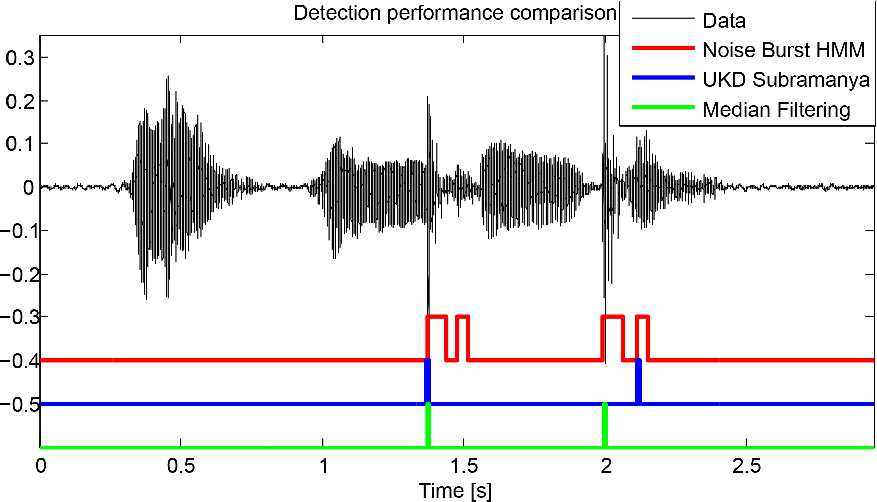
\includegraphics[width=12cm]{NBDetCompare.pdf}
  \begin{picture}(0,0)
%\put(-310,275){a)}
%\put(-310,135){b)}
\end{picture}}
\end{minipage}
\caption{Comparison of Noise Burst detection algorithm on mixed signal.}
\label{fig:NBDetCompare.pdf}
\end{figure}

To quantify the performance of the algorithms, the test performed in \ref{fig:NBDetCompare.pdf} was run on the two audio sequences seen in Figure~\ref{fig:res}. Figure~\ref{fig:res}(a) shows the results from running the algorithm on 10 clean keystrokes, and Figure~\ref{fig:res}(b) shows the results from 10 keystrokes but each of which are embedded at different points in different utterances. The algorithms are all tuned to be as sensitive as possible on a third audio sequence containing 8 seconds of only speech without getting any detections.

To further quantify the performance of the algorithm a similar test to the above was run on 61 seconds of speech and 43 individual keyboards taps. The audio was recorded via an external microphone in 16kHz and all algorithms were tuned similarly to the previous test. The results of this test has been tabulated in Table~\ref{table:resultsTest}.

\begin{table}
\caption{Detection results}
\centering
\begin{tabular}{|l | c c c|}
\hline
                            & Noise Burst   & UKD       & Median        \\
 \hline
 Correct detection rate     & 34 \%         & 20 \%     & 50 \%         \\
 False detections pr second & 0             & 0.03      & 0.02          \\
 \hline
 \end{tabular}
 \label{table:NBResultsTest}
\end{table}

It is clear from Figure~\ref{fig:NBDetectionResults} and Table~\ref{table:NBResultsTest} that both the Noise Burst and the UKD algorithm outperform the standard median filter approach. Figure~\ref{fig:NBDetectionResults}(a) shows the UKD algorithm being slightly more sensitive than the Noise Burst model, while in Figure~\ref{fig:NBDetectionResults}(b) the UKD appears slightly less sensitive to embedded taps while finding more false detections than the Noise Burst model. Table~\ref{table:NBResultsTest} shows the Noise Burst algorithm being more sensitive than UKD while all tested algorithms maintain a low false detection rate. The median detector's good performance in the last test is probably explained by the relatively loud transients in the audio compared to the speech.


\begin{figure}
\begin{minipage}[b]{1.0\linewidth}
  \centering
  \centerline{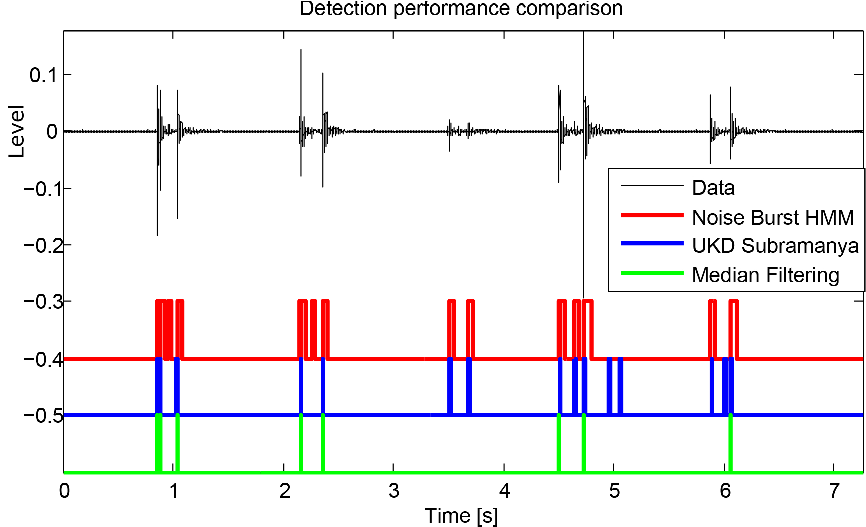
\includegraphics[width=12.5cm]{NBDetCompareLongTaps}}
%  \vspace{2.0cm}
  \centerline{(a) 10 taps with no speech.}\medskip
\end{minipage}
%
\begin{minipage}[b]{1.0\linewidth}
  \centering
  \centerline{\includegraphics[width=12.5cm]{NBDetCompareLongTapsnTalk}}
%  \vspace{1.5cm}
  \centerline{(b) 10 taps embedded in 10 utterances. Stars indicate ground truth.}\medskip
\end{minipage}
\hfill
%
\caption{Detection results for sequences of taps.}
\label{fig:NBDetectionResults}
\end{figure}

\subsection{AR filtering approach}

The terminal node coefficients of the WPT of an incoming audio sequence $x(n)$ of length $N$ is defined as $X(j,t)$ where $j$ is the $j$th terminal node, $j \in \{1, \ldots, J\}$, and $t$ is the time index related to $n$. A level $L$ WPT gives $J = 2^L$ terminal nodes. $X(t)$ will be used to denote a vector of all coefficients at a given time index $t$. We assume that the coefficients for each terminal node $j$ follow this linear predictive model

\begin{equation}\label{eq:lpm}
X(j,t) = \sum_{m=1}^{M} a_{j,m} X(j,t - m) + v(j,t),
\end{equation}

where $a_{jm}$ is the $m$th weight applied to the $j$th terminal node so that $\mathbf{a}_j = \{a_{j,1}, \ldots, a_{j,M} \}$, $M$ is the size of the buffer used, and $v(j,t)$ is Gaussian noise with zero mean so that

\begin{equation}\label{eq:lpmnoise}
v(j,t) \sim \mathcal{N}_v(0,\sigma^2_{j,t}).
\end{equation}

We can now express the probability of $X(j,t)$ conditional on prior values of $X$.

\begin{align}\label{eq:likelihood}
p\left(X\left(j,t\right)|X\left(j,t-1\right),\ldots,X\left(j,t-M\right)\right) = \nonumber\\
\qquad \mathcal{N}_X\left( \sum_{m=1}^M a_{j,m} X(j,t - m), \sigma_{j,t}^2\right),
\end{align}

and the marginal probability can be expressed as

\begin{equation}\label{eq:marginal}
p\left(X(t)\right) = \prod^J p\left(X(j,t)\right),
\end{equation}

assuming that the conditional probabilities for each set of coefficients are independent.

We can now calculate the log-likelihood $\log\mathcal{L} = \log{p\left(X(t)\right)}$ for the current coefficient $X(t)$,

\begin{align}\label{eq:loglike}
\log \mathcal{L} &= \log \left\{ \prod^J p \left( X(j,t) | X(j,t-1),\ldots,X(j,t-M) \right) \right\} \\
&=  \sum^J \log \left\{p \left( X(j,t) | X(j,t-1),\ldots,X(j,t-M) \right) \right\}\nonumber\\
&=  -\frac{1}{2} \sum^J \frac{1}{\sigma_{j,t}^2}\left(X(j,t) -  \sum_{m=1}^{M} a_{j,m} X(j,t - m) \right)^2 + C_{j,t}\nonumber,
\end{align}
where $C_{j,t}$ is a constant. The value $\log \mathcal{L}$ is now a measure of how well $X(t)$ can be predicted by its previous values.

\subsubsection{Results}
\todo{Fill out this section}


% ------------------------------------------------------------------------


%%% Local Variables:
%%% mode: latex
%%% TeX-master: "../thesis"
%%% End:
